

\tikzset{every picture/.style={line width=0.75pt}} %set default line width to 0.75pt        

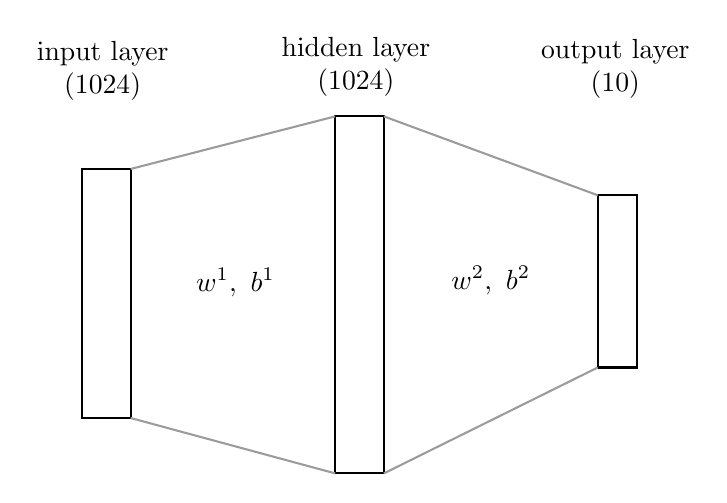
\begin{tikzpicture}[x=0.75pt,y=0.75pt,yscale=-1,xscale=1]
%uncomment if require: \path (0,300); %set diagram left start at 0, and has height of 300

%Shape: Rectangle [id:dp6149643085998178] 
\draw   (54,93.33) -- (77.5,93.33) -- (77.5,213.33) -- (54,213.33) -- cycle ;
%Shape: Rectangle [id:dp5092925997669449] 
\draw   (176,68) -- (199.5,68) -- (199.5,240) -- (176,240) -- cycle ;
%Straight Lines [id:da7027489864850467] 
\draw [color={rgb, 255:red, 155; green, 155; blue, 155 }  ,draw opacity=1 ]   (77.5,93.33) -- (176,68) ;


%Straight Lines [id:da30180540366043385] 
\draw [color={rgb, 255:red, 155; green, 155; blue, 155 }  ,draw opacity=1 ]   (77.5,213.33) -- (176,240) ;


%Shape: Rectangle [id:dp4986098264860639] 
\draw   (302.5,106) -- (321.5,106) -- (321.5,189) -- (302.5,189) -- cycle ;
%Straight Lines [id:da45051042505798455] 
\draw [color={rgb, 255:red, 155; green, 155; blue, 155 }  ,draw opacity=1 ]   (199.5,68) -- (302.5,106) ;


%Straight Lines [id:da9299225224259415] 
\draw [color={rgb, 255:red, 155; green, 155; blue, 155 }  ,draw opacity=1 ]   (199.5,240) -- (302.5,189) ;



% Text Node
\draw (128,148) node  [align=left] {$\displaystyle w^{1} ,\ b^{1}$};
% Text Node
\draw (251,147) node  [align=left] {$\displaystyle w^{2} ,\ b^{2}$};
% Text Node
\draw (186,44) node  [align=center] {hidden layer\\(1024)};
% Text Node
\draw (64,46) node  [align=center] {input layer\\(1024)};
% Text Node
\draw (311,45) node  [align=center] {output layer\\(10)};


\end{tikzpicture}
